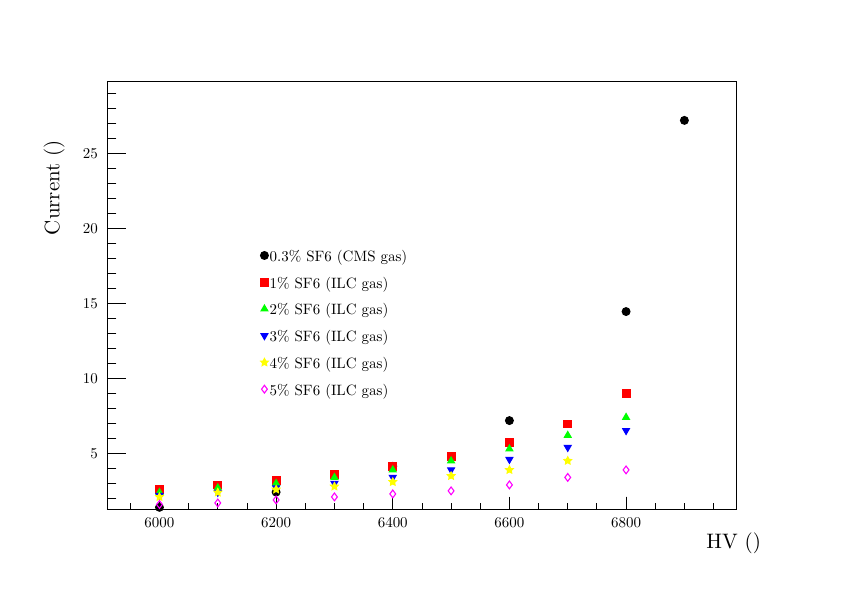
\begin{tikzpicture}
\pgfdeclareplotmark{cross} {
\pgfpathmoveto{\pgfpoint{-0.3\pgfplotmarksize}{\pgfplotmarksize}}
\pgfpathlineto{\pgfpoint{+0.3\pgfplotmarksize}{\pgfplotmarksize}}
\pgfpathlineto{\pgfpoint{+0.3\pgfplotmarksize}{0.3\pgfplotmarksize}}
\pgfpathlineto{\pgfpoint{+1\pgfplotmarksize}{0.3\pgfplotmarksize}}
\pgfpathlineto{\pgfpoint{+1\pgfplotmarksize}{-0.3\pgfplotmarksize}}
\pgfpathlineto{\pgfpoint{+0.3\pgfplotmarksize}{-0.3\pgfplotmarksize}}
\pgfpathlineto{\pgfpoint{+0.3\pgfplotmarksize}{-1.\pgfplotmarksize}}
\pgfpathlineto{\pgfpoint{-0.3\pgfplotmarksize}{-1.\pgfplotmarksize}}
\pgfpathlineto{\pgfpoint{-0.3\pgfplotmarksize}{-0.3\pgfplotmarksize}}
\pgfpathlineto{\pgfpoint{-1.\pgfplotmarksize}{-0.3\pgfplotmarksize}}
\pgfpathlineto{\pgfpoint{-1.\pgfplotmarksize}{0.3\pgfplotmarksize}}
\pgfpathlineto{\pgfpoint{-0.3\pgfplotmarksize}{0.3\pgfplotmarksize}}
\pgfpathclose
\pgfusepathqstroke
}
\pgfdeclareplotmark{cross*} {
\pgfpathmoveto{\pgfpoint{-0.3\pgfplotmarksize}{\pgfplotmarksize}}
\pgfpathlineto{\pgfpoint{+0.3\pgfplotmarksize}{\pgfplotmarksize}}
\pgfpathlineto{\pgfpoint{+0.3\pgfplotmarksize}{0.3\pgfplotmarksize}}
\pgfpathlineto{\pgfpoint{+1\pgfplotmarksize}{0.3\pgfplotmarksize}}
\pgfpathlineto{\pgfpoint{+1\pgfplotmarksize}{-0.3\pgfplotmarksize}}
\pgfpathlineto{\pgfpoint{+0.3\pgfplotmarksize}{-0.3\pgfplotmarksize}}
\pgfpathlineto{\pgfpoint{+0.3\pgfplotmarksize}{-1.\pgfplotmarksize}}
\pgfpathlineto{\pgfpoint{-0.3\pgfplotmarksize}{-1.\pgfplotmarksize}}
\pgfpathlineto{\pgfpoint{-0.3\pgfplotmarksize}{-0.3\pgfplotmarksize}}
\pgfpathlineto{\pgfpoint{-1.\pgfplotmarksize}{-0.3\pgfplotmarksize}}
\pgfpathlineto{\pgfpoint{-1.\pgfplotmarksize}{0.3\pgfplotmarksize}}
\pgfpathlineto{\pgfpoint{-0.3\pgfplotmarksize}{0.3\pgfplotmarksize}}
\pgfpathclose
\pgfusepathqfillstroke
}
\pgfdeclareplotmark{newstar} {
\pgfpathmoveto{\pgfqpoint{0pt}{\pgfplotmarksize}}
\pgfpathlineto{\pgfqpointpolar{44}{0.5\pgfplotmarksize}}
\pgfpathlineto{\pgfqpointpolar{18}{\pgfplotmarksize}}
\pgfpathlineto{\pgfqpointpolar{-20}{0.5\pgfplotmarksize}}
\pgfpathlineto{\pgfqpointpolar{-54}{\pgfplotmarksize}}
\pgfpathlineto{\pgfqpointpolar{-90}{0.5\pgfplotmarksize}}
\pgfpathlineto{\pgfqpointpolar{234}{\pgfplotmarksize}}
\pgfpathlineto{\pgfqpointpolar{198}{0.5\pgfplotmarksize}}
\pgfpathlineto{\pgfqpointpolar{162}{\pgfplotmarksize}}
\pgfpathlineto{\pgfqpointpolar{134}{0.5\pgfplotmarksize}}
\pgfpathclose
\pgfusepathqstroke
}
\pgfdeclareplotmark{newstar*} {
\pgfpathmoveto{\pgfqpoint{0pt}{\pgfplotmarksize}}
\pgfpathlineto{\pgfqpointpolar{44}{0.5\pgfplotmarksize}}
\pgfpathlineto{\pgfqpointpolar{18}{\pgfplotmarksize}}
\pgfpathlineto{\pgfqpointpolar{-20}{0.5\pgfplotmarksize}}
\pgfpathlineto{\pgfqpointpolar{-54}{\pgfplotmarksize}}
\pgfpathlineto{\pgfqpointpolar{-90}{0.5\pgfplotmarksize}}
\pgfpathlineto{\pgfqpointpolar{234}{\pgfplotmarksize}}
\pgfpathlineto{\pgfqpointpolar{198}{0.5\pgfplotmarksize}}
\pgfpathlineto{\pgfqpointpolar{162}{\pgfplotmarksize}}
\pgfpathlineto{\pgfqpointpolar{134}{0.5\pgfplotmarksize}}
\pgfpathclose
\pgfusepathqfillstroke
}
\definecolor{c}{rgb}{1,1,1};
\draw [color=c, fill=c] (0,0) rectangle (10,6.79083);
\draw [color=c, fill=c] (1,0.679083) rectangle (9,6.11175);
\definecolor{c}{rgb}{0,0,0};
\draw [c,line width=0.3] (1,0.679083) -- (1,6.11175) -- (9,6.11175) -- (9,0.679083) -- (1,0.679083);
\draw [c,line width=0.3] (1,0.679083) -- (9,0.679083);
\draw [c,line width=0.3] (1.66667,0.842063) -- (1.66667,0.679083);
\draw [c,line width=0.3] (2.03704,0.760573) -- (2.03704,0.679083);
\draw [c,line width=0.3] (2.40741,0.760573) -- (2.40741,0.679083);
\draw [c,line width=0.3] (2.77778,0.760573) -- (2.77778,0.679083);
\draw [c,line width=0.3] (3.14815,0.842063) -- (3.14815,0.679083);
\draw [c,line width=0.3] (3.51852,0.760573) -- (3.51852,0.679083);
\draw [c,line width=0.3] (3.88889,0.760573) -- (3.88889,0.679083);
\draw [c,line width=0.3] (4.25926,0.760573) -- (4.25926,0.679083);
\draw [c,line width=0.3] (4.62963,0.842063) -- (4.62963,0.679083);
\draw [c,line width=0.3] (5,0.760573) -- (5,0.679083);
\draw [c,line width=0.3] (5.37037,0.760573) -- (5.37037,0.679083);
\draw [c,line width=0.3] (5.74074,0.760573) -- (5.74074,0.679083);
\draw [c,line width=0.3] (6.11111,0.842063) -- (6.11111,0.679083);
\draw [c,line width=0.3] (6.48148,0.760573) -- (6.48148,0.679083);
\draw [c,line width=0.3] (6.85185,0.760573) -- (6.85185,0.679083);
\draw [c,line width=0.3] (7.22222,0.760573) -- (7.22222,0.679083);
\draw [c,line width=0.3] (7.59259,0.842063) -- (7.59259,0.679083);
\draw [c,line width=0.3] (1.66667,0.842063) -- (1.66667,0.679083);
\draw [c,line width=0.3] (1.2963,0.760573) -- (1.2963,0.679083);
\draw [c,line width=0.3] (7.59259,0.842063) -- (7.59259,0.679083);
\draw [c,line width=0.3] (7.96296,0.760573) -- (7.96296,0.679083);
\draw [c,line width=0.3] (8.33333,0.760573) -- (8.33333,0.679083);
\draw [c,line width=0.3] (8.7037,0.760573) -- (8.7037,0.679083);
\draw [anchor=base] (1.66667,0.454986) node[scale=0.540924, color=c, rotate=0]{6000};
\draw [anchor=base] (3.14815,0.454986) node[scale=0.540924, color=c, rotate=0]{6200};
\draw [anchor=base] (4.62963,0.454986) node[scale=0.540924, color=c, rotate=0]{6400};
\draw [anchor=base] (6.11111,0.454986) node[scale=0.540924, color=c, rotate=0]{6600};
\draw [anchor=base] (7.59259,0.454986) node[scale=0.540924, color=c, rotate=0]{6800};
\draw [c,line width=0.3] (1,0.679083) -- (1,6.11175);
\draw [c,line width=0.3] (1.24,1.39093) -- (1,1.39093);
\draw [c,line width=0.3] (1.12,1.58155) -- (1,1.58155);
\draw [c,line width=0.3] (1.12,1.77217) -- (1,1.77217);
\draw [c,line width=0.3] (1.12,1.96279) -- (1,1.96279);
\draw [c,line width=0.3] (1.12,2.15341) -- (1,2.15341);
\draw [c,line width=0.3] (1.24,2.34403) -- (1,2.34403);
\draw [c,line width=0.3] (1.12,2.53465) -- (1,2.53465);
\draw [c,line width=0.3] (1.12,2.72527) -- (1,2.72527);
\draw [c,line width=0.3] (1.12,2.91589) -- (1,2.91589);
\draw [c,line width=0.3] (1.12,3.10651) -- (1,3.10651);
\draw [c,line width=0.3] (1.24,3.29713) -- (1,3.29713);
\draw [c,line width=0.3] (1.12,3.48775) -- (1,3.48775);
\draw [c,line width=0.3] (1.12,3.67837) -- (1,3.67837);
\draw [c,line width=0.3] (1.12,3.86899) -- (1,3.86899);
\draw [c,line width=0.3] (1.12,4.05961) -- (1,4.05961);
\draw [c,line width=0.3] (1.24,4.25023) -- (1,4.25023);
\draw [c,line width=0.3] (1.12,4.44085) -- (1,4.44085);
\draw [c,line width=0.3] (1.12,4.63147) -- (1,4.63147);
\draw [c,line width=0.3] (1.12,4.82209) -- (1,4.82209);
\draw [c,line width=0.3] (1.12,5.01271) -- (1,5.01271);
\draw [c,line width=0.3] (1.24,5.20333) -- (1,5.20333);
\draw [c,line width=0.3] (1.24,1.39093) -- (1,1.39093);
\draw [c,line width=0.3] (1.12,1.20031) -- (1,1.20031);
\draw [c,line width=0.3] (1.12,1.00969) -- (1,1.00969);
\draw [c,line width=0.3] (1.12,0.81907) -- (1,0.81907);
\draw [c,line width=0.3] (1.24,5.20333) -- (1,5.20333);
\draw [c,line width=0.3] (1.12,5.39395) -- (1,5.39395);
\draw [c,line width=0.3] (1.12,5.58457) -- (1,5.58457);
\draw [c,line width=0.3] (1.12,5.77518) -- (1,5.77518);
\draw [c,line width=0.3] (1.12,5.9658) -- (1,5.9658);
\draw [anchor= east] (0.95,1.39093) node[scale=0.540924, color=c, rotate=0]{5};
\draw [anchor= east] (0.95,2.34403) node[scale=0.540924, color=c, rotate=0]{10};
\draw [anchor= east] (0.95,3.29713) node[scale=0.540924, color=c, rotate=0]{15};
\draw [anchor= east] (0.95,4.25023) node[scale=0.540924, color=c, rotate=0]{20};
\draw [anchor= east] (0.95,5.20333) node[scale=0.540924, color=c, rotate=0]{25};
\foreach \P in {(1.66667,0.705889), (3.14815,0.899487), (4.62963,1.22712), (6.11111,1.80791), (7.59259,3.19252), (8.33333,5.62031)}{\draw[mark options={color=c,fill=c},mark size=1.402402pt,mark=*] plot coordinates {\P};}
\definecolor{c}{rgb}{1,0,0};
\foreach \P in {(1.66667,0.933441), (2.40741,0.990627), (3.14815,1.04781), (3.88889,1.12406), (4.62963,1.21937), (5.37037,1.35281), (6.11111,1.52818), (6.85185,1.76454), (7.59259,2.15627)}{\draw[mark options={color=c,fill=c},mark
 size=1.402402pt,mark=square*] plot coordinates {\P};}
\definecolor{c}{rgb}{0,1,0};
\foreach \P in {(1.66667,0.895317), (2.40741,0.952503), (3.14815,1.00969), (3.88889,1.08594), (4.62963,1.18125), (5.37037,1.29562), (6.11111,1.44811), (6.85185,1.61967), (7.59259,1.84842)}{\draw[mark options={color=c,fill=c},mark
 size=1.402402pt,mark=triangle*] plot coordinates {\P};}
\definecolor{c}{rgb}{0,0,1};
\foreach \P in {(1.66667,0.857194), (2.40741,0.896271), (3.14815,0.953457), (3.88889,1.01064), (4.62963,1.08689), (5.37037,1.1822), (6.11111,1.31468), (6.85185,1.46718), (7.59259,1.68162)}{\draw[mark options={color=c,fill=c,rotate=180},mark
 size=1.402402pt,mark=triangle*] plot coordinates {\P};}
\definecolor{c}{rgb}{1,1,0};
\foreach \P in {(1.66667,0.838132), (2.40741,0.895317), (3.14815,0.933441), (3.88889,0.971565), (4.62963,1.02875), (5.37037,1.105), (6.11111,1.18125), (6.85185,1.29753)}{\draw[mark options={color=c,fill=c},mark size=1.402402pt,mark=newstar*] plot
 coordinates {\P};}
\definecolor{c}{rgb}{1,0,1};
\foreach \P in {(1.66667,0.742822), (2.40741,0.761884), (3.14815,0.800008), (3.88889,0.838132), (4.62963,0.876256), (5.37037,0.915333), (6.11111,0.990627), (6.85185,1.08594), (7.59259,1.18125)}{\draw[mark options={color=c,fill=c},mark
 size=1.402402pt,mark=diamond] plot coordinates {\P};}
\definecolor{c}{rgb}{1,1,1};
\draw [color=c, fill=c] (3,2.03725) rectangle (3,4.0745);
\definecolor{c}{rgb}{0,0,0};
\draw [anchor=base west] (3,3.82833) node[scale=0.540924, color=c, rotate=0]{   0.3\% SF6 (CMS gas)};
\foreach \P in {(3,3.90473)}{\draw[mark options={color=c,fill=c},mark size=1.402402pt,mark=*] plot coordinates {\P};}
\draw [anchor=base west] (3,3.48879) node[scale=0.540924, color=c, rotate=0]{   1\% SF6 (ILC gas)};
\definecolor{c}{rgb}{1,0,0};
\foreach \P in {(3,3.56519)}{\draw[mark options={color=c,fill=c},mark size=1.402402pt,mark=square*] plot coordinates {\P};}
\definecolor{c}{rgb}{0,0,0};
\draw [anchor=base west] (3,3.14925) node[scale=0.540924, color=c, rotate=0]{   2\% SF6 (ILC gas)};
\definecolor{c}{rgb}{0,1,0};
\foreach \P in {(3,3.22564)}{\draw[mark options={color=c,fill=c},mark size=1.402402pt,mark=triangle*] plot coordinates {\P};}
\definecolor{c}{rgb}{0,0,0};
\draw [anchor=base west] (3,2.80971) node[scale=0.540924, color=c, rotate=0]{   3\% SF6 (ILC gas)};
\definecolor{c}{rgb}{0,0,1};
\foreach \P in {(3,2.8861)}{\draw[mark options={color=c,fill=c,rotate=180},mark size=1.402402pt,mark=triangle*] plot coordinates {\P};}
\definecolor{c}{rgb}{0,0,0};
\draw [anchor=base west] (3,2.47016) node[scale=0.540924, color=c, rotate=0]{   4\% SF6 (ILC gas)};
\definecolor{c}{rgb}{1,1,0};
\foreach \P in {(3,2.54656)}{\draw[mark options={color=c,fill=c},mark size=1.402402pt,mark=newstar*] plot coordinates {\P};}
\definecolor{c}{rgb}{0,0,0};
\draw [anchor=base west] (3,2.13062) node[scale=0.540924, color=c, rotate=0]{   5\% SF6 (ILC gas)};
\definecolor{c}{rgb}{1,0,1};
\foreach \P in {(3,2.20702)}{\draw[mark options={color=c,fill=c},mark size=1.402402pt,mark=diamond] plot coordinates {\P};}
\definecolor{c}{rgb}{0,0,0};
\draw [anchor= east] (0.328,5.46393) node[scale=0.756643, color=c, rotate=90]{Current (\si{\micro\ampere})};
\draw [anchor= east] (9.4,0.250766) node[scale=0.756643, color=c, rotate=0]{HV (\si{\volt})};
\end{tikzpicture}
